\documentclass[a4paper, 12pt]{report}

\usepackage[finnish]{babel}         % Suomenkielinen tavutus
\usepackage[fixlanguage]{babelbib}
\selectbiblanguage{finnish}
\usepackage[utf8x]{inputenc}
\usepackage{ifpdf}
\usepackage{graphicx}
% load tocbibind package 
%   - do not include table of contents in itself
%   - convert the name of bibliography to references
\usepackage[nottoc]{tocbibind}

% load sverb package
%   - enhanced handling of verbatim stuff; listing environment
\usepackage{sverb}

% load listings package
%   - handle inclusion of source code
\usepackage{listings}

% load fancyheaders package
%   - the actual headers and footers are set later
\usepackage{fancyhdr}

% load itpackage 
%   - additional defines and stuff
\usepackage{thesis/itpackage}

\usepackage{enumitem}

\usepackage{hyperref}

\title{JavaScriptin staattinen tyypittäminen}
\author{Oskari Noppa \\kandidaatintutkielma \\ tietojenkäsittelytiede \\ Turun yliopisto}
\date{Lokakuu 2017}

\begin{document}
  \selectlanguage{finnish}\fintrue

  \iffin
  \settocbibname{Lähdeluettelo}
  \renewcommand{\appname}{Liitteet}
  \else
  \settocbibname{References}
  \renewcommand{\appname}{Appendices}
  \fi
  
  % Fill in your information below
  \workinfo{Oskari Noppa}
  {JavaScriptin staattinen tyypittäminen}
  {Jari-Matti Mäkelä}
  {Second Supervisor}
  {2017}
  {10}
  {Lokakuu}
  
  % Set the type of your thesis (Diplomityö, TkK -tutkielma, etc.) and
  % laboratory or field of study below
  \worktype{}{LuK -tutkielma} 
  \deptinfo{}{Tietojenkäsittelytiede}
  
  % Generate the title page 
  \gentitle
  
  % empty pagestyle for table of contents etc. 
  %
  % the redefinition of plain style works also for 1st pages of chapters,
  % which is the default in report class. Just state \thispagestyle{empty}
  % after \chapter{something} if you want empty style for the 1st pages. 
  %
  \pagestyle{empty}
  \fancypagestyle{plain}{
    \fancyhf{}
    \renewcommand{\headrulewidth}{0 pt}
  }
  
  % roman numbering for table of contents etc.
  \pagenumbering{roman}
  
  % insert table of contents, list of figures, list of tables
  %
  % setting the counter to zero effectively removes the page number from
  % the toc, lof etc. entries in the toc since there is no roman numeral
  % for zero ;-) (if you want them without numbering)
  %
  %\setcounter{page}{0}
  \tableofcontents
  \clearpage
  %\setcounter{page}{0}
  %\listoffigures 
  %\clearpage
  %\setcounter{page}{0}
  %\listoftables
  
  % possibly insert 'list of acronyms'
  %
  %   - create a chapter called List Of Acronyms (or whatever), which
  %     should contain all your acronym definitions, e.g. 
  %     \chapter{List Of Acronyms} 
  %   - the secnumdepth trickery is needed because acronyms are as a
  %     standard chapter and we are faking '\listofacronyms'
  %
  %\setcounter{secnumdepth}{-1}
  %\input{your acronym chapter's file name}
  %\setcounter{secnumdepth}{2}
  
  % setup page numbering, page counter, etc.
  \startpages
  
  \chapter{Johdanto} \label{Johdanto}

Ohjelmointi on pohjimmiltaan tietorakenteiden käsittelyä ja yksi tärkeimmistä
tietorakenteen ominaisuuksista on sen tyyppi. Muuttuja “nimi” voi olla
datatyypiltään teksti ja muuttuja “ikä” voi olla numero, eikä näitä kahta voi
huolettomasti sekoittaa. Ohjelman tila ei ole järkevä jos se sanoo henkilön
iän olevan “Matti”. Se miten ohjelmointikielissä käsitellään arvojen tyyppejä
vaihtelee kuitenkin suuresti.

Tässä tutkielmassa käsitellään JavaScriptiä, sekä kolmea työkalua jotka
lisäävät rakentavat staattisesti tarkastettavan tyyppijärjestelmän
JavaScriptin päälle. JavaScript on dynaamisesti tyypitetty ohjelmointikieli,
jonka alkuperäinen käyttötarkoitus oli lisätä verkkosivuille pieniä
interaktiivisia ominaisuuksia, kuten lomakkeiden validointia. JavaScriptillä
toteutettavien ohjelmien koko, monimutkaisuus ja tärkeys on kuitenkin viime
vuosien aikana kasvanut alkuperäistä tarkoitusperää suuremmaksi, kun sillä on
alettu toteuttaa esimerkiksi kartta-, kirjoitus- ja hallintapalveluita jotka
toimivat selaimessa, siten ettei käyttäjän tarvitse asentaa erillistä
ohjelmaa palvelun käyttöön.

Tutkielmassa esitellään TypeScript, Flow ja Closure-kääntäjä, joista jokainen on
kehitetty työkaluksi parempien JavaScript-ohjelmien kehittämiseksi.
Tarkastelussa ilmenee, että staattinen tyypitys voi nopeuttaa ohjelman
kehittämistä, vähentää ohjelmoijan tekemien virheiden määrää ja parantaa
valmiin ohjelman tehokkuutta. Toisaalta nähdään myös, että valinta staattisen
ja dynaamisen tyypityksen välillä sisältää kompromisseja, etenkin kun
tyyppijärjestelmä on erillinen työkalu eikä kieleen alusta asti kehitetty
ominaisuus.

  \chapter{Peruskäsitteitä}

\section{Tyyppijärjestelmien luokitteleminen}
Ohjelmointikielten tyyppijärjestelmien jakaminen staattisesti ja dynaamisesti
tyyppitarkastettuihin perustuu ohjelman kehitysvaiheeseen jossa tarkastaminen
tapahtuu. Staattisella tyyppitarkastamisella viitataan ohjelman tyyppien
analyysiin ennen sen suorittamista, esimerkiksi käännösaikana, kun taas
dynaaminen tyyppitarkastus varmistaa arvojen tyyppien oikeellisuuden ohjelmaa
suoritettaessa. Tyyppijärjestelmät voidaan jaotella myös muiden
ominaisuuksien perusteella, esimerkiksi vahvoihin ja heikkoihin
tyyppijärjestelmiin. Näiden termien merkitys ei ole tarkasti määritelty,
mutta yleisesti niillä viitataan tapaan jolla kieli käsittelee tarkoitetusta
poikkeavat, virheelliset tyypit \cite{CornellTransitionToOO}. Vahvasti
tyypitetyssä kielessä tällainen aiheuttaisi käännös- tai ajonaikaisen
virheen, kun taas heikosti tyypitetyssä kielessä arvoille voitaisiin tehdä
implisiittisiä tyyppimuunnoksia niiden yhteensopivuuden saavuttamiseksi.

JavaScript on dynaamisesti tarkastettu, heikosti tyypitetty kieli.
Esimerkiksi ohjelma \inlinecode{\dblquoted{teksti}.potenssiin(3)} antaa
staattisesti tyyppitarkastetussa kielessä virheen jo käännösaikana, mikäli
metodia \inlinecode{potenssiin} ei ole tekstityyppisille arvoille määritetty.
JavaScriptiä suorittava ympäristö sen sijaan hyväksyisi ohjelman ja sallisi
sen suorittamisen. Virhe olemattoman metodin kutsumisesta ilmenisi vasta jos
ohjelman suoritus evaluoi kyseisen ilmaisun. Lisäksi esimerkiksi ilmaisu
\inlinecode{\dblquoted{teksti} + 2} ei aiheuttaisi virhettä edes 
suoritusaikana, sillä heikoille tyyppijärjestelmille ominaisesti JavaScript
muuttaisi numeron 2 string-muotoon ennen summausoperaation arviointia. Tässä
tutkielmassa keskitytään lähinnä JavaScriptin tyyppien staattiseen ja
dynaamiseen, eli käytännössä käännös- ja ajonaikaiseen tarkastamiseen. Jotkin
esitellyistä työkaluista myös tiukentavat kielen sallimia operaatioita siten,
että esimerkiksi yllä esitettyä \inlinecode{\dblquoted{teksti} + 2} ohjelmaa
ei enää sallittaisi. Monia muita heikoille tyyppijärjestelmille
tavallisia ominaisuuksia jää kuitenkin tarkistamatta.

\begin{figure}
\centering
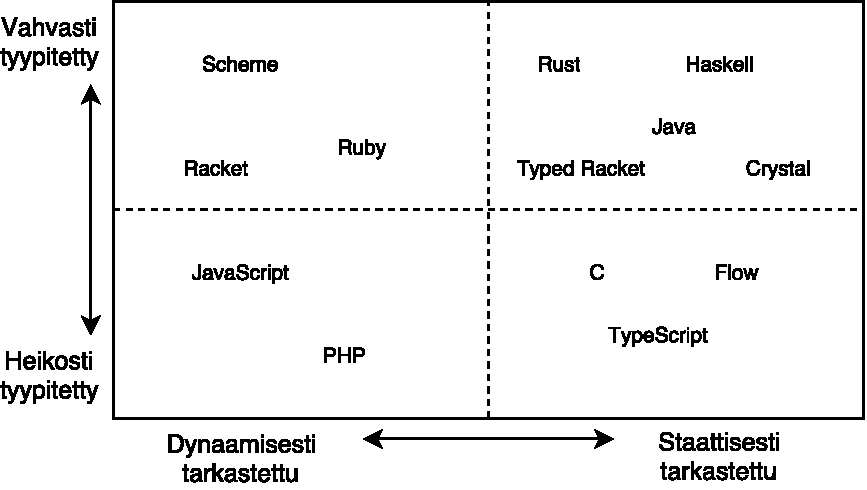
\includegraphics{images/type-systems.pdf}
\caption{Tyyppijärjestelmät eri ohjelmointikielissä}
\end{figure}

\section{ECMA-262, EcmaScript ja JavaScript}
``EcmaScript'' on ECMA-262 standardin määrittelemä ohjelmointikieli
\cite{JavaScriptLanguageResources}\cite{Ecma262}, jonka kehityksestä vastaa
organisaatio Ecma International. ``JavaScript'' on Oraclen omistama
tavaramerkki jolla viitataan EcmaScript-kielen osittaisiin tai täydellisiin
toteutuksiin.[4] Historiallisista syistä termejä
``JavaScript'' ja ``EcmaScript'' käytetään usein keskenään vaihtokelpoisesti.
Tässä tutkielmassa termillä ``JavaScript'' viitataan ECMA-262:den kahdeksannen
version mukaiseen EcmaScriptiin, jota kutsutaan myös nimellä EcmaScript 2017.

\section{TypeScript}
TypeScript on Microsoftin luoma ohjelmointikieli, jonka tarkoitus on
auttaa JavaScript-ohjelmien kehitystä staattisen tyyppijärjestelmän avulla.
Se on EcmaScriptin ylijoukko (superset) \cite{TypeScriptSpec} ja jatkaa
JavaScriptin syntaksia tyyppimäärittelyihin käytettävällä
annotaatiosyntaksilla. Jokainen validi JavaScript-ohjelma on syntaksiltaan ja
ajonaikaiselta käyttäytymiseltään validi TypeScript-ohjelma. TypeScript
kuitenkin lisää kehitykseen käännösvaiheen, jossa ohjelman tyyppien
oikeellisuus tarkastetaan staattisesti. TypeScript koodi käännetään
JavaScriptiksi, joka puolestaan voidaan suorittaa selaimissa tai muissa
JavaScriptin suoritusympäristöissä. TypeScript kääntäjän voi myös määrittää
muokkaamaan tulostettava koodi yhteensopivaksi vanhempien
EcmaScript-standardien kanssa, mikä on hyödyllistä jos ohjelman on tarkoitus
tukea sellaisia suoritusympäristöjä jotka eivät tue uusinta EcmaScriptin
versiota.

\section{Flow}
Flow on Facebookin kehittämä työkalu, joka TypeScriptin tavoin jatkaa
JavaScriptin syntaksia staattisesti tarkastettavilla tyyppimäärittelyillä.
Flow itsessään ei sisällä kääntäjää, vaan keskittyy yksinomaan ohjelman
tyyppiturvallisuuden tarkastamiseen. Koodiin lisätyt tyyppimääritykset on
kuitenkin poistettava ennen kuin JavaScript-ohjelma voidaan suorittaa. Tähän
tarkoitukseen voidaan käyttää esimerkiksi Babel-kääntäjää, joka poistaa
Flow-tyyppimäärittelyt ja muokkaa JavaScript-koodin yhteensopivaksi toivotun
EcmaScript-version kanssa \cite{FlowInstallation}.

\section{Closure kääntäjä}
Googlen Closure kääntäjä on käännöstyökalu, jonka pääasiallinen tarkoitus
on minimoida ja optimoida JavaScript-koodia käännösvaiheessa ennen tuotantoon
siirtämistä. Closure sisältää kuitenkin myös tuen tyyppivirheiden
tarkastamiselle käännösvaiheessa \cite{ClosureCompiler}. Tyypit annotoidaan
erityisellä JSDoc-pohjaisilla dokumentaatiokommenteilla. Koska annotaatiot
ovat kommenteissa eivätkä erityisenä syntaksina muun suoritettavan koodin
joukossa, Closure-annotoitua JavaScriptiä ei tarvitse kääntää ennen sen
suorittamista \cite{annotatingJSforClosure}.
  \chapter{Työkalun käyttöönotto}

\section{Tyyppiannotaatiot}

Tyyppijärjestelmä voi päätellä muuttujan sallitun tyypin automaattisesti
päättelemällä tai kieleen sisältyvien eksplisiittisten tyyppimäärittelyjen
perusteella. SML kykenee tulkitsemaan kaikkien muuttujien arvot
automaattisesti, kun taas Java vaatii kaikkien olevan eksplisiittisesti
annotoituja. Suurin osa staattisesti tyyppitarkastetuista kielistä kuitenkin
putoaa jonnekkin välimaastoon. Haskell, C\#, Crystal ja monet muut tarjoavat
syntaksin tyyppien eksplisiittiselle määrittämiselle mutta tarjoavat myös
kielikohtaisesti vaihtelevan tuen tyyppien automaattiselle päättelylle. Tässä
on hyvä huomioida että vaikka tyyppien tulkinta tapahtuu automaattisesti,
niin se suoritetaan tässä tapauksessa silti käännös- eikä suoritusaikana.
Esimerkiksi yllä mainittu Crystal on tarvittavien annotaatioiden vähyydestä
huolimatta staattisesti tyyppitarkastettu, toisin kuin syntaksin inspiraation
lähteenä ollut Ruby.

Kaikki kolme tässä esiteltyä JavaScriptin staattiseen tyyppitarkastukseen
tarkoitettua työkalua päättelevät tyyppejä automaattisesti, mutta vaativat
myös eksplisiittisiä määrityksiä paikoitellen. Closure-kääntäjä lukee
tyyppimääritykset JSDoc-tyylisistä dokumentaatiokommenteista. TypeScript ja
Flow puolestaan jatkavat ECMA-262 -spesifikaatiota erityisellä syntaksilla
tyyppien eksplisiittistä määrittelyä varten. Kumpikaan näistä
lähestymistavoista ei ole täysin ongelmaton. Dokumentaatiokommentit voivat
olla hankala ja ”verbose” formaatti monimutkaisille tyyppiannotaatioille,
mikä kasvattaa niiden kirjoittamiseen vaadittua työmäärää. [Hejlsberg quote].
Toisaalta jo opitun JavaScriptin syntaksin jatkaminen uudella syntaksilla
vaatii uusien merkintöjen oppimmista ja saattaa vaikeuttaa kirjoitetun koodin
lukemista etenkin tottumattomille lukijoille.

\section{Ohjelman kääntäminen ennen suorittamista}

JavaScript koodi tulkataan tai käännetään tyypillisesti suorittamisen
yhteydessä, selaimesta tai muusta suoritusympäristöstä löytyvän ”moottorin”
toimesta. EcmaScript standardin mukaista koodia suorittamaan suunnitellut
moottorit, kuten V8 tai SpiderMonkey, eivät kuitenkaan osaa käsitellä
TypeScript- tai Flow-annotaatioilla merkattua koodia. Näinollen TypeScript-
tai Flow-annotoitu koodi on välttämätöntä [sivuhuomio] kääntää muotoon jossa
annotaatiot on poistettu ja jäljellä on enää standardinmukainen JavaScript.
Koska JavaScriptin käyttäminen ei normaalisti vaadi erillistä
käännösvaihetta, useissa projekteissa ei ole sellaista käytetty. Koodin
minimointi ja muu optimointi on ollut parhaiden käytäntöjen mukaista jo
tovin, mutta tällaiset koodinkäsittelyt tehdään yleensä vasta ennen koodin
julkaisua. Kehittäjät ovat tavanomaisesti voineet suorittaa kirjoittamansa
JavaScriptin sellaisenaan kehitysympäristössä. Käännösvaiheen aikavaatimus
pyritään luonnollisesti pitämään mahdollisimman pienenä, mutta se on silti
projektin monimutkaisuuteen ja kehitysnopeuteen vaikuttava tekijä joka
työkalun käyttöönotossa tulee huomioida.
  \chapter{Virheiden havaitseminen}

Kenties tärkein staattisen tyyppijärjestelmän tehtävä on havaita ja estää
ohjelmoijan virheitä. Tässä esitellyt työkalut, mahdollisesti Closure
kääntäjää lukuunottamatta, onkin kehitetty erityisesti tätä tarkoitusta
varten.

Kaikki kolme työkalua antaisivat käännösvirheen jos esimerkeissä
\ref{lst:ostoskorin_hinta_clojure} ja \ref{lst:ostoskorin_hinta_flow}
esiteltyä funktiota kutsuttaisiin virheellisesti esimerkiksi listalla
hintaa kuvaavia numeroita, sillä funktion parametrin on annotoitu olevan
lista ``Ostos''-tyyppimääritelmän mukaisia objekteja. Esimerkiksi
virheellinen kutsu
\colorbox{lightgray}{\lstinline|ostoskorinHinta([5, 10, 15])|} ei itse
asiassa aiheuttaisi suoritettaessa ohjelman keskeyttävää virhettä.
\colorbox{lightgray}{\lstinline|ostos.hinta|} ilmaisu on sallittu vaikka
muuttuja \colorbox{lightgray}{\lstinline|ostos|} olisikin arvoltaan numero
eikä objekti. Tällöin ilmaisun arvo on \colorbox{lightgray}{\lstinline|undefined|}
ja lausekkeen \colorbox{lightgray}{\lstinline|summa += ostos.hinta|} jälkeen
\colorbox{lightgray}{\lstinline|summa|} muuttujan arvo on erityinen
ei-numeroa kuvaava \colorbox{lightgray}{\lstinline|NaN|} \cite{Ecma262NaN}.
Käännösaikaisen tarkistamisen merkitys korostuu erityisen hyödylliseksi
tämänkaltaisen ohjelmointivirheen kohdalla, sillä virhe ei välttämättä ole
muutoin helposti havaittavissa. Funktiokutsu ei aiheuttaisi helposti
todennettavaa suoritusaikaista virhettä, joten ei-toivottu palautusarvo
\colorbox{lightgray}{\lstinline|NaN|} saattaisi kiertää ohjelman
operaatioiden välillä pitkällekin aiheuttaen muita loogisia virheitä.

  \chapter{Ohjelman optimointi käännösvaiheessa staattisen analyysin perusteella}


  \chapter{Tyyppimäärittelyt dokumentaationa}
  \chapter{Ongelmat JavaScriptin staattisessa tyypittämisessä}

\section{Luotettavuus, täydellisyys ja käytännöllisyys}

\begin{figure}
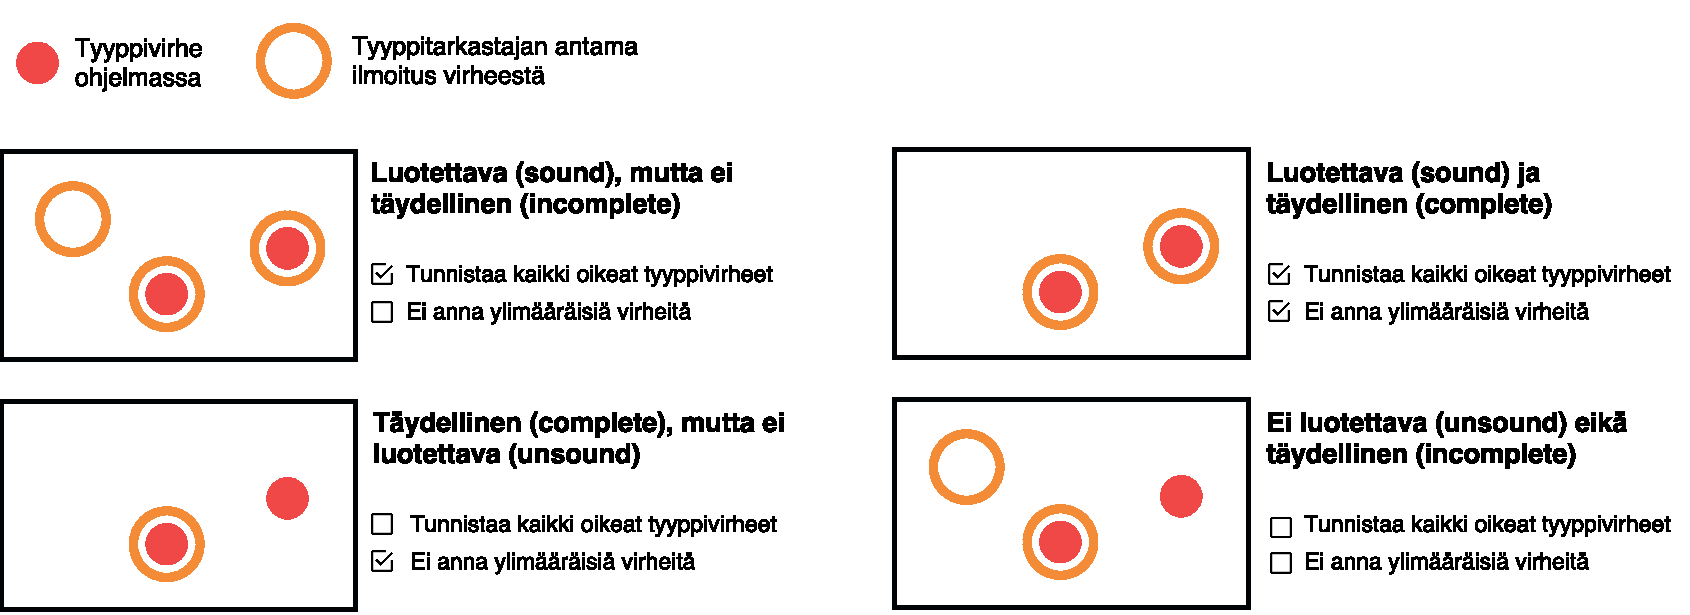
\includegraphics[width=\textwidth]{images/soundness_completeness2.pdf}
\caption{Tyyppijärjestelmän luotettavuus ja täydellisyys}
\end{figure}

Tyyppijärjestelmän luotettavuus (soundness) kuvaa sitä, kuinka suuren osan
mahdollisista ohjelmointivirheistä se estää. Täysin luotettava (sound)
tyyppijärjestelmä estää kaikki sellaiset virheet jotka sen on tarkoitus
estää \cite{CSE_ProgrammingLanguages}. Täydellisyys (completeness)
puolestaan kertoo salliiko tyyppijärjestelmä kielen sellaiset ominaisuudet
jotka eivät olisi ajonaikana tyyppivirheitä \cite{TypesAndProgrammingLanguages, CSE_ProgrammingLanguages}.

Jotta JavaScriptiä analysoiva tyyppijärjestelmä olisi luotettava, sen on
annettava virhe esimerkiksi seuraavasta ohjelmasta:

\begin{minipage}{\linewidth}
\begin{lstlisting}[caption={Virheellinen JavaScript-ohjelma: Lisätyllä tuotteella ei ole nimeä.}]
function osta(ostos) {
  lisaaTuote({
    nimi: ostos.nimi,
    hinta: ostos.hinta
  });
}

osta({ nimi: 'juusto', hinta: 5 });
osta({ hinta: 5 });
\end{lstlisting}
\label{fig:soundness_test}
\end{minipage}

Toisaalta jotta JavaScriptiä analysoiva tyyppijärjestelmä olisi täydellinen,
sen on sallittava tämä korjattu versio ylläolevasta ohjelmasta:

\begin{minipage}{\linewidth}
\begin{lstlisting}[caption={Toimiva JavaScript-ohjelma: Virheelliseltä kutsulta on suojauduttu tarkistuksella.}]
function osta(ostos) {
  if (typeof ostos.nimi === 'string') {
    lisaaTuote({
      nimi: ostos.nimi,
      hinta: ostos.hinta
    });
  }
}

osta({ nimi: 'juusto', hinta: 5 });
osta({ hinta: 5 });
\end{lstlisting}
\label{fig:completeness_test}
\end{minipage}

Esimerkit \ref{fig:soundness_test} ja \ref{fig:completeness_test} toimivat
odotetulla tavalla Flow:ssa. TypeScript vaatii eksplisiittisen tyyppiannotaation
osta-funktiolle, mutta toimii muuten samalla tavalla.


  \chapter{Yhteenveto}

Tyyppijärjestelmä on tärkeä ohjelmointikielen ominaisuus, jolla on suuri
vaikutus ohjelmistokehittäjän käyttökokemukseen.
Liian tiukka tyyppijärjestelmä voi rajoittaa sitä mitä kielellä voi tehdä,
sillä harva tyyppijärjestelmä on täydellinen (engl. complete).
Ohjelmointikielissä on usein ominaisuuksia joissa esimerkiksi merkkijonon
odotettu arvo on riippuvainen ohjelman rajapinnoista ja suoritusaikaisista
rakenteista, mutta joita tutkielmassa esitetyt tekniikat tai
monimutkaisemmatkaan tyyppijärjestelmät eivät välttämättä kykene
kuvaamaan ja tarkistamaan.

Lisäksi eksplisiittiset tyyppimäärittelyt vaativat lisää kirjoitettavaa
koodia kun funktioiden parametrien ja luokkien jäsenmuuttujien tyyppikuvaukset
tulee kirjoittaa kommentteihin (Closure) tai tyyppiannotaatioiksi
(TypeScript ja Flow).
Eksplisiittisistä tyyppimäärittelyistä voi olla hyötyä
koodin dokumentaationa, mutta kehittäjä saattaa myös kokea niiden
kirjoittamisen rasitteena. Dynaamisesti tyypitettyä koodia on usein
nopeampi tuottaa ja iteroida etenkin kehitysprosessin alkuvaiheissa, jolloin
käytettyjen tyyppien rakenne voi muuttua useaan kertaan. 

Dynaamisesti tyypitetyn koodin nopeasta kirjoitustahdista saatavat hyödyt jäävät kuitenkin
vähäisiksi jos lopputuotos ei toimi odotetulla tavalla. Ohjelmistovirheet heikentävät
käyttäjien tyytyväisyyttä ohjelmaan ja voivat pahimmillaan aiheuttaa
pysyvää vahinkoa saadessaan ohjelman toimimaan virheellisesti.
Staattinen tyypitys ohjaa kirjoitettua koodia turvalliseen suuntaan kehitysvaiheen alusta
loppuun ja torjuu tietynlaisia ohjelmointivirheitä tehokkaammin kuin
esimerkiksi ajonaikaista käyttäytymistä testaavat yksikkötestit.

Tässä tutkielmassa on esitelty kolme työkalua, jotka lisäävät dynaamisesti
tyypitettyyn JavaScriptiin käännösaikaisen tyyppitarkastuksen sekä syntaksin
tyyppien eksplisiittiseen määrittämiseen. Flow, TypeScript ja Closure
sallivat asteittaisen siirtymisen dynaamisesti tyyppitarkastetusta staattisesti
tarkastettuun, sekä staattisen tarkastuksen ohittamisen niissä osissa koodia
joihin sitä olisi liian vaikeaa tai mahdotonta lisätä.
Samankaltaisuus ja yhteensopivuus jo ennestään suositun JavaScriptin kanssa
yhdistettynä tyyppiturvallisuuteen, koodin kirjoittamista helpottaviin
työkaluihin ja selkeämmin dokumentoituun koodiin ovat nostaneet erityisesti
TypeScriptin käytön nopeaan kasvuun.


  \bibliographystyle{thesis/unsrtf}
  \bibliography{bibliografia}
  
  % make sure pagecount is correct even if references overflow to a new page
  \pagebreak\addtocounter{page}{-1}
  \eofpages
  \appendices
  
  % create your appendix chapters with command \appchapter{some name} instead
  % of \chapter{some name} for the automagic page counting to work
  %\input{file name of appchapter xxx}
  %\input{file name of appchapter yyy}
  %\input{file name of appchapter zzz}
  %\input{and so on}
  
  \eofapppages


\end{document}
